%%%%%%%%%%%%%%%%%%%%%%%%%%%%%%%%%%%%%%%%%%%%%%%%%%%%%%%%%%%%%%%%%%%%%%%%%%%%%%%%
%2345678901234567890123456789012345678901234567890123456789012345678901234567890
%        1         2         3         4         5         6         7         8
\documentclass[letterpaper, 10pt, conference]{ieeeconf}      % Use this line for a4 paper

\IEEEoverridecommandlockouts                              % This command is only needed if 
                                                          % you want to use the \thanks command

\overrideIEEEmargins                                      % Needed to meet printer requirements.

% See the \addtolength command later in the file to balance the column lengths
% on the last page of the document

\usepackage[utf8x]{inputenc}

\usepackage[protrusion=true,expansion=true]{microtype}
\usepackage{cite}
\usepackage{graphicx}
\usepackage{hyperref}
\usepackage{url}
\usepackage{amsmath}
\usepackage{booktabs}

\usepackage[cache]{minted}
\renewcommand{\theFancyVerbLine}{
  \sffamily\textcolor[rgb]{0.5,0.5,0.5}{\scriptsize\arabic{FancyVerbLine}}}

\newminted{python}{frame=lines,
                    linenos=true,
                    gobble=4,
                    fontsize=\scriptsize,
                    xleftmargin=1.8em}

\newmintinline[python]{python}{fontsize=\footnotesize}

\graphicspath{{figs/}}
\DeclareGraphicsExtensions{.pdf,.jpg,.png}

\usepackage[draft]{fixme}

\newcommand{\ie}{{\textit{i.e.\ }}}
\newcommand{\cf}{{\textit{cf\ }}}
\newcommand{\eg}{{\textit{e.g.\ }}}
\newcommand{\pyRobots}{\textsc{pyRobots}}


\title{\LARGE \bf
    \pyRobots{}, a toolset for robot executive control
}

\author{Séverin Lemaignan, Anahita Hosseini and Pierre Dillenbourg\\
Computer-Human Interaction in Learning and Instruction \\
École Polytechnique Fédérale de Lausanne (EPFL) \\
CH-1015 Lausanne, Switzerland \\
{\tt\small firstname.last@epfl.ch}
}

\begin{document}


\maketitle
\thispagestyle{empty}
\pagestyle{empty}


%%%%%%%%%%%%%%%%%%%%%%%%%%%%%%%%%%%%%%%%%%%%%%%%%%%%%%%%%%%%%%%%%%%%%%%%%%%%%%%%
\begin{abstract}

Presented is \pyRobots{}, a new open-source software toolkit for the executive
control of complex robotic systems. Borrowing ideas from previous tools like
{\sc urbi}~\cite{baillie2005urbi}, it proposes a lightweight Python framework to
develop (pre-emptive) concurrent and event-based executive controllers.

Designed in a \emph{bottom-up} fashion, out of the need for a practical,
unobstrusive tool suitable for rapid prototyping of complex interaction
scenarios, \pyRobots{} also exposes several simple yet convenient abstractions
for physical resources management and pose representation. While
middleware-agnostic, it features specific integration with the ROS middleware.

Experimental deployments and stress-tests on several robotic platforms
(including PR2 and Nao) in dynamic human environments are reported.

\end{abstract}


%%%%%%%%%%%%%%%%%%%%%%%%%%%%%%%%%%%%%%%%%%%%%%%%%%%%%%%%%%%%%%%%%%%%%%%%%%%%%%%%
\section{Introduction}

Orchestrating the activity of a robot is a central issue of robotics: \emph{what
to do when?} Traditionally, in layered architectures, this function is
implemented in the so-called \emph{deliberative layer} where decisions are made
based on perceptions and on the current internal state, and executed by sending
orders to a \emph{functional layer}.

While individual decision-making components (such as task planners) have been
studied in (relative) isolation for decades, the \emph{orchestration} issue,
with questions such as \textit{When to start them? Which one should be selected?
How to react to a new situation in a timely manner?} remains difficult to
address in a generic way.

Many approaches have been devised that
include \emph{Finite State Machines} (FSM), domain-specific languages (in
particular, logic languages) or agent-based frameworks; these are reviewed in
the next section.

These tools adopt principled approaches, often with solid theoretical
contributions. However, it seems that none of them gained broad acceptance in
the robotic community, and many of us resort to write ad-hoc scripts, suitable
for a single application/demonstration/experiment and neither reliable nor
extensible. We hypothesize that the software architecture that these tools
enforce, combined with their general lack of practicality (unfamiliar language;
lack of bindings for a given robot or middleware; difficulty to install or
setup; non-trivial deployment) explain this low level of acceptance more than
any particular intrinsic weaknesses.

This article introduces our attempt at designing an unobtrusive execution
control toolset that aims at addressing the \emph{practicality} issue: it has
been designed and implemented from the bottom-up, starting from actual needs
when running large robotic systems (including robots such as PR2 or Nao) in
dynamic and partially unpredictable environments, such as loosely constrained
human-robot interaction scenarios.

Instead of an \emph{environment} or a \emph{framework}, which would suggest
rigid design and development guidelines, \pyRobots{} can be conceived as a set
of software libraries to write parallel, event-based, high-level robot
controllers.  It is written for and in Python, which ensure familiarity, fast
development cycles and broad support for interfacing with existing robots and
middlewares. \pyRobots{} is indeed \emph{not} a middleware: it purposefully
provides no mechanisms to connect to other modules or components. It instead
\emph{relies} on one (or several) middleware(s) to actually communicate with the
robot.

\subsection{Related Work: Robot Execution Control}

Any robotic experiment requires a certain amount of high-level control to
supervise the robot behaviour, and, expectedly, many projects have attempted to
design and provide tools for this task. Degroote provides an in-depth review of
the existing techniques and tools in~\cite{degroote2012architecture}. We focus
this review on tools dedicated to the explicit implementation of high-level
behaviours, excluding complete control stacks (that would typically include a
middleware and hardware abstractions), meta-tools (such as component generators
or model checkers) and (semi-)automatic techniques (such as emerging behaviours
or learning by demonstration). Unlike \emph{middlewares} where a few tools --
ROS, YARP, {\sc orocos}-rtt, OpenRTM -- are the \emph{de facto} standards, no tool really
dominates the field of execution control, and we believe instead that most of
today's robot behaviours are implemented as \emph{ad-hoc} scripts.

We identify three categories of execution control tools: \emph{finite state
machines}, \emph{agent-based} controllers and
\emph{Domain-Specific Languages} (DSL), including \emph{embedded Domain-Specific
Languages} (eDSL,~\cite{joyeux2011robot}). These categories overlap to a certain
extent, but still reflect reasonably well the motivational concepts/ideas that
gave birth to the specific tools.

\paragraph{Finite State Machines} They are the most well-known paradigm to
describe how a robot goes from one \emph{state} (typically, performing an
action) to another state when some condition is satisfied or some event is
triggered. Common FSM implementations in robotics include {\sc
rfSM}~\cite{klotzbucher2010orocos} (part of the {\sc orocos} framework) and
{\sc smach}~\cite{bohren2010smach}. State machine semantics are well
understood~\cite{harel1996statemate} and provide a well structured model,
suitable for meta-reasoning (such as verification). However, FSM are also
acknowledged to be ill-suited for complex systems (where the number of state
easily ``explodes'') or relatively dynamic and unpredictable environments where
it can prove difficult to exhaustively list transitions \textit{a priori}.


\paragraph{Agent-based controllers}

The T-REX architecture~\cite{mcgann2007trex} partitions the execution control
problem into several agents, each one composed of a (temporal) planner and an
execution layer. At run-time, the different agents are constantly synchronised
to maintain the consistency of the global plan. ROAR~\cite{degroote2011roar}
augments this idea with a logic mechanism, allowing the system to automatically
select and start agents depending on the task at hand.

\paragraph{Domain-specific languages}

In the broadest sense, they represent the largest body of literature on
high-level behaviour programming. They can either be actual domain-specific
languages such as PRS~\cite{ingrand1996prs}, RPL~\cite{mcdermott1993reactive},
Golog~\cite{levesque1997golog} (and its derivatives such as {\sc
ReadyLOG}~\cite{ferrein2007robot}) or, more recently, {\sc
urbi}~\cite{baillie2005urbi}; or what Joyeux calls \emph{embedded}
DSL~\cite{joyeux2011robot}. eDSL are extensions of existing languages (typically, dynamic
languages such as Python or Ruby, or logic languages such as Prolog) to provide
high-level paradigms and control structures well suited to the programming of
robots. {\sc cram}~\cite{beetz2010cram} (based on Lisp and Prolog), {\sc
roby}~\cite{joyeux2009plan} (based on Ruby), {\sc teer}~\cite{magnenat2012teer}
(based on Python), are examples of such eDSL.

\pyRobots{} positions itself in this landscape as a lightweight eDSL (in a
similar fashion to {\sc roby} or {\sc teer}), that focuses on high-level
behaviour implementation. Unlike larger stacks, \pyRobots{} does not provide
formal models or verifiability. It aims to provide unobtrusive interaction with
the other components of the robot software stack, using Python as the ubiquitous
binding language. Similar to {\sc urbi}, it focuses on transparent pre-emptive
concurrency and event-based programming.  Also, \pyRobots{}' model favours
hierarchical task composition over plans, and does not provide by itself any
task planning service.

%\subsection{Guiding principles}
%
%\begin{itemize}
%    \item Use a de-facto standard language (Python) to ease adoption (familiar to
%        many researchers, large software ecosystem, excellent integration with
%        most robotic softwares, in particular common middlewares like ROS or
%        YARP)
%    \item should be as lightweight/transparent as possible (in particular from a
%        syntax perspective) so that the
%        programmer can focus on the programming of the behaviours (I'm
%        watching you, SMACH)
%    \item should enforce as few design choices as possible. 'convention over
%        configuration' as often as possible
%\end{itemize}
%
%\subsection{Main features}
%
%Parallelism (all \emph{actions} are asynchronous) and event-based programming
%are at the core.
%
%It also offers support for robot resources management (locking of ``parts'' of
%the robot) and uniform manipulation of 6D poses (that integrates transparently
%with other tools like ROS's {\sc tf} when available).
%
\section{Concepts and Overview}

This section introduces the main concepts of \pyRobots{}, and provide an
overview of the features and mechanisms. The interested reader can refer to
the source code and documentation, available
from~\url{https://github.com/chili-epfl/pyrobots}.

\subsection{Core concepts}

\pyRobots{} core concepts are simple: on one hand, the user creates a
\textbf{robot} as an instance of a \python|GenericRobot| that encapsulates the
different low-level \textbf{controllers} (proxies to actuators, typically
provided by a middleware such as ROS) and the \textbf{state} of the robot
(typically a set of proxies to the sensors accessed through a key-value
container).

On the other hand, the user creates as many high-level \textbf{actions} as
desired, as regular Python functions, only annotated with the \python|@action|
decorator. Actions are automatically added to the \textbf{robot}, and can access
its state and controllers to perform actual physical actions.

The user can list \textbf{events} that the \textbf{robot} must monitor, and
attach callbacks to them.

Finally, the user can declare arbitrary \textbf{resources}, usually
corresponding to the robot's physical components (for instance, the wheels, the
camera) and guarantee exclusive access to these resource to a specific set of
actions.

\subsection{Asynchronous actions}

\emph{Actions} in \pyRobots{} are asynchronous by default. They are implemented as
\emph{futures} (also known as \emph{promises}) and therefore executed in
independent threads. To the developer, however, they appear as regular Python
functions annotated with the \python|@action| decorator, and are invoked
like any other function.  Since they are asynchronous, these functions may
block or even never return (typically useful for implementing continuous
background behaviours).

Actions can also call each other (nested actions), allowing natural
decomposition of complex tasks into sub-actions (the nesting depth of an action
is hereafter noted $depth$).

Behaviours often need to be paused or cancelled.  This raises
an issue that specifically needs to be addressed in robotics: before suspending
an action, one often wants to first bring back the robot into some form of rest
state (\eg one would not want to suddenly cancel a \python|walk| action in the
middle of a step without first bringing back the foot to the ground). \pyRobots{}
addresses this issue through signals, and extends the standard Python thread into
\emph{signaling threads}, relying on Python's usual syntax for exception
handling. Listing~\ref{lst:signals} illustrates this mechanism. The action is
instantiated and started at line 8, and cancelled at line 10. This sends an
\python|ActionCancelled| signal to the action that the user can handle using an
\python|except| statement.

\begin{listing}
\begin{pythoncode}
    @action
    def safe_walk(robot):
      try:
        robot.walk()
      except ActionCancelled:
        robot.go_back_to_rest_pose()

    action = robot.safe_walk()
    time.sleep(1)
    action.cancel()
\end{pythoncode}
\caption{\textbf{Handling a cancellation signal} After one second, the
\python|safe_walk| action is cancelled. This sends the signal
\python|ActionCancelled| to the action that can appropriately handle it inside
the \python|except| block.}
\label{lst:signals}
\end{listing}

Pausing actions is more complex (the action's internal state must be saved, a
means to resume the action must be provided and the user must be given ways to
code transition behaviours when pausing and resuming) and is not currently
supported by \pyRobots{}.

\subsection{Events}

Sharing the same syntax with {\sc urbi}, events in \pyRobots{} can by monitored
through the methods \python|on| (one shot event) and \python|whenever|
(continuous event monitoring). Event conditions can either be a predicate
(taking the robot instance as its only argument) or a $\{\text{state
key}, \text{condition}\}$ pair, with condition one of $\{\text{value}=x,
\text{below}=x, \text{above}=x, \text{decrease}=x, \text{increase}=x\}$.
Examples of event usage can be seen at lines 33--38 of
listing~\ref{croquignole_no_move}.

Each event monitor lives in its own separate thread, and when the event is fired,
the callback (usually, an action) is invoked from the event monitor thread
itself.

\subsection{Resource management}

Physical robot resources (mainly actuators, but possibly sensors as
well) usually mandate exclusive use. \pyRobots{} provides a resource
locking mechanism that relies on the \python|@lock| annotation: an action
annotated with \python|@lock(ARMS)| (Listing~\ref{lst:resources}, l.6) will
acquire (or wait for) the \python|ARMS| resource before being executed.

This mechanism is generic and \pyRobots{} makes no assumptions concerning the
actual resources available to a specific robot. The
programmer define them himself, either as stand-alone or as compound
resources (Listing~\ref{lst:resources}, l.1--3).

A given action can lock several distinct resources with the corresponding
number of \python|@lock| annotations. When executed, the
action acquires a lock on the resource (and all sub-resources in the case
of a compound resource) which is released upon action completion. If the lock is
already acquired, two strategies are possible: either wait or \emph{fail fast}
(\python|@lock(..., wait=False)|, Listing~\ref{lst:resources}, l.16).

\begin{listing}
\begin{pythoncode}
    L_ARM = Resource()
    R_ARM = Resource()
    ARMS = CompoundResource(L_ARM, R_ARM)

    @action
    @lock(ARMS)
    def lift_box(robot):
        #...

    @action
    @lock(L_ARM)
    def wave_hand(robot):
        #...

    @action
    @lock(L_ARM, wait=False)
    def scratch_head(robot):
        #...

    robot.lift_box()
    robot.wave_hand() # waits until lift_box is over
    robot.scratch_head() # skipped if lift_box or
                         # wave_hand are still running

\end{pythoncode}
\caption{\textbf{Resource locking} Resource usage is defined at the
action-level, through annotations.}

\label{lst:resources}
\end{listing}



\subsection{Uniform management of poses and rigid transformations}

Managing poses, transformations and frames in real-world scenarios is not an
easy task, mainly because it appears that libraries, middlewares or robotic
platforms tend each to rely on their own conventions; rotation representations,
in particular, are a common source of inconsistencies -- quaternions, Euler
conventions, rotation matrices, Rodrigues, yaw-pitch-roll notations being all
rather frequent. Within the ROS ecosystem, the Transform Library ({\sc
tf},~\cite{foote2013tf}) has played a major role in making it convenient to work
with frames: poses can always be expressed and shared in the most convenient
local frame, {\sc tf} taking care of required intermediate transformation.

\pyRobots{} pose management builds on this idea to offer flexible pose
representations \emph{within} the control scripts. Every time a 6D pose needs to
be specified (like a navigation goal or a target pose for an arm), it can be
expressed as a simple frame name, by a 3-tuple $(x, y, z)$ (default frame {\tt
map} is then assumed), by a 4-tuple $(x, y, z, frame)$, by a 6-tuple $(x, y, z,
rx, ry, rz)$ (using $sxyz$ Euler convention), by a 7-tuple $(x, y, z, rx, ry,
rz, frame)$, by a 7-tuple $(x, y, z, qx, qy, qz, qw)$, by an 8-tuple $(x, y, z,
qx, qy, qz, qw, frame)$ or by a dictionary that defines any subset of $(x, y, z,
qx, qy, qz, qw, frame)$.  Internally, \pyRobots{} normalizes and stores the
poses in their full 8-tuple expansion, as illustrated in
Listing~\ref{lst:poses}.

\begin{listing}
    \begin{pythoncode*}{linenos=false, xleftmargin=0em}

    robot.poses["handL"]
    # -> {'x':0., 'y':0., 'z':0., 
    #    'qx':0., 'qy':0., 'qz':0., 'qw':1., 
    #    'frame': 'handL'}

    robot.poses[(1.0, 0.0, 0.0)]
    # -> {'x':1., 'y':0., 'z':0., 
    #    'qx':0., 'qy':0., 'qz':0., 'qw':1., 
    #    'frame': 'map'}

    robot.poses[{'z':1.0, 'rz':0.2, 'frame':'handL'}]
    # -> {'x':0., 'y':0., 'z':1., 
    #    'qx':0., 'qy':0., 'qz':0.0998, 'qw':0.0995, 
    #    'frame': 'handL'}

\end{pythoncode*}
\caption{Examples of \textbf{pose normalization}. Poses can be transformed to
other reference frames with the \python|inframe| method (which implicitly performs
normalization if needed).}
\label{lst:poses}
\end{listing}

Using helper methods such as \python|inframe| \python|(<pose>, <other frame>)| or
\python|pantilt| \python|(<pose>, <ref frame>)|, the programmer can then
transform a given pose into a different frame or different representation.

Required transformations are computed by \pyRobots{}, and the programmer can
provide new ``sources'' of frame transformations through the instantiation of
\python|FrameProviders| that takes advantage of robot- and middleware-specific
infrastructures (for example, ROS {\sc tf}, Aldebaran's {\tt NAOqi} frame
conventions, etc.).

\subsection{Developer support: logging, debugging, introspection}
\label{}

Running robots in real-world  environments that are dynamic and unpredictable
entails repetitive coding-testing-debugging development cycles. \pyRobots{}
provides several tools to support this development phase that rely on the
versatile Python built-in logging tools, which support configurable parallel
logging streams (typically, a full debug stream is logged to a file while a less
verbose stream is output on the console at run-time).

\pyRobots{} logs are designed to allow full \emph{offline} replay, and we
provide a graphical interface to display the actions and resource usage over
time (Figure~\ref{log_view}).

\begin{figure}
        \centering
        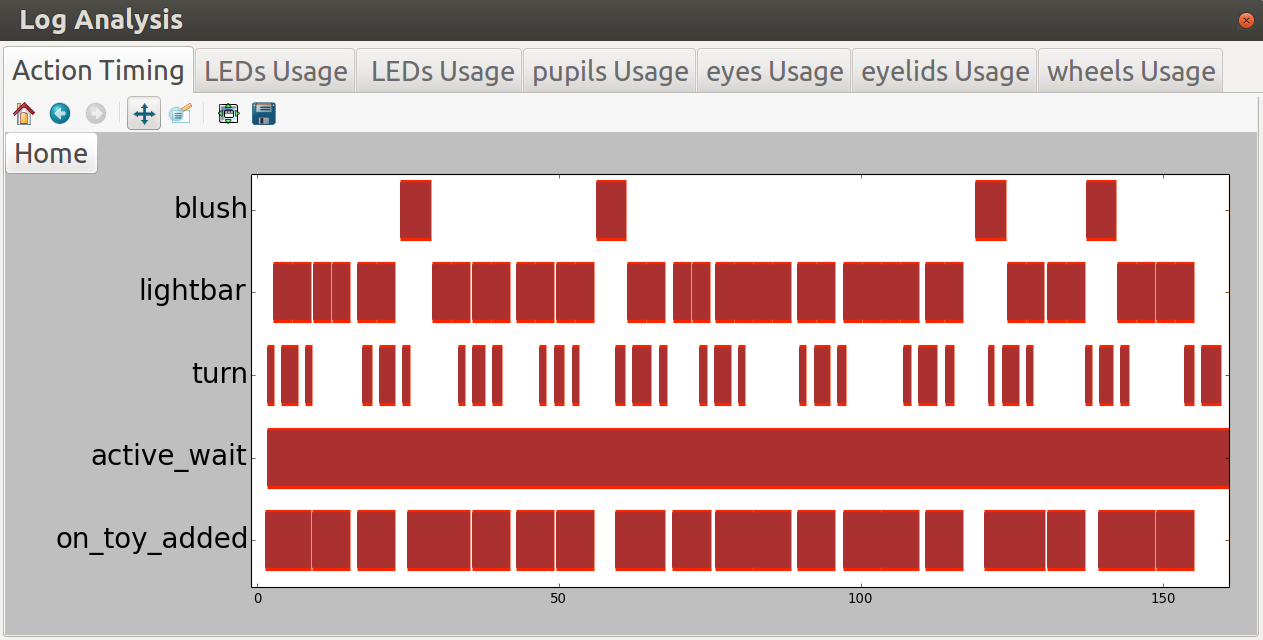
\includegraphics[width=0.9\columnwidth]{log}
        \caption{Screenshot of \pyRobots{} log analyzer, processing the log of the
        experiment presented in section~\ref{croq}}
        \label{log_view}
\end{figure}

Debugging and introspection support is provided at run-time through a range of
off-the-shelf Python debuggers. Remote debugging is also supported with standard
tools such as {\sc rpdb2}~\footnote{\url{http://winpdb.org}}. Python being an
interpreted language, these debuggers do not only provide insights on failures,
but also tooling for full introspection and run-time manipulation of the
application state.

%%%%%%%%%%%%%%%%%%%%%%%%%%%%%%%%%%%%%%%%%%%%%%%%%%%%%%%%%%%%%%%%%%%%%%%%%%%%%%

\section{Experimental Deployments}

The development of \pyRobots{} started in 2011, driven by the requirements of a
18min long theatre performance between a human actor and a robot. Since that
time, the toolset has iteratively matured, and has been deployed and used on
several projects and platforms. We first briefly summarize these deployments,
and then present a recent study in a kindergarten that acted as a stress-test
for the library.

\begin{table}[h]
    \centering
    \begin{tabular}{lll}
        \toprule
        Study                 & Robot & Middlewares \\ \midrule
        Roboscopie            & PR2       & ROS, {\sc GenoM} \\
        Interactive Grounding & PR2, LAAS-CNRS's Jido & ROS, {\sc GenoM} \\
        CoWriter              & Nao       & ROS, NAOqi  \\
        Ranger at kindergarten & EPFL's Ranger & ROS, aseba  \\
        \bottomrule
    \end{tabular}
    \caption{Overview of the main studies where \pyRobots{} was used.}
\end{table}

\subsubsection{Roboscopie} The first complex deployment scenario for \pyRobots{} was
a theatre performance entitled \emph{Roboscopie}~\cite{lemaignan2012roboscopie}.
The toolset was created out of the need to control a complex robot (a PR2) in a structured way, as required for a live performance with a
human\footnote{The original \pyRobots{} script used for the performance can be
accessed from~\url{http://www.laas.fr/roboscopie}. Note that this script does
not reflect anymore the current toolkit usage.}.

A total of 47 \pyRobots{} actions were written for this event
(Table~\ref{pyrobots_actions} gives a few significant examples), and the toolset
proved to be convenient for interleaving calls to both ROS-based and
{\sc GenoM}-based~\cite{mallet2010genom3} components through their respective
Python bindings.

\pyRobots{} also allowed us to retain the \emph{rapid prototyping} convenience
of a script language, essential for the robot's programmer to quickly adapt to
the vision of the director.

%%%%%%%%%%%%%%%%%%%%%%%%%%%%%%%%%%%%%%%%%%%%%%%%%%%%
\begin{table}[ht!]
\begin{center}
\begin{tabular}{p{0.9\columnwidth}}
    \toprule
    {\bf Manipulation} \\
     {\tt attachobject}, {\tt basicgive}, {\tt basictake}, {\tt close\_gripper}, {\tt configure\_grippers}, {\tt grab\_gripper}, {\tt handover}, {\tt hide}, {\tt open\_gripper}, {\tt pick}, {\tt put}, {\tt put\_accessible}, {\tt release\_gripper}, {\tt show}, {\tt take} \\
     \midrule
    {\bf Gaze control} \\
     {\tt glance\_to}, {\tt look\_at}, {\tt sweep}, {\tt switch\_active\_stereo\_pair}, {\tt track}, {\tt cancel\_track} \\
     \midrule
    {\bf Navigation} \\
     {\tt carry}, {\tt follow}, {\tt cancel\_follow}, {\tt goto}, {\tt moveclose}, {\tt waypoints} \\
     \midrule
    {\bf Local navigation} \\
     {\tt dock}, {\tt rotate}, {\tt translate} \\
     \midrule
    {\bf Posture configuration} \\
     {\tt extractpose}, {\tt idle}, {\tt manipose}, {\tt movearm}, {\tt rest}, {\tt setpose}, {\tt settorso}, {\tt tuckedpose} \\
     \bottomrule
\end{tabular}
\end{center}
\caption{Examples of \pyRobots{} actions.}

\label{pyrobots_actions}
\end{table}
%%%%%%%%%%%%%%%%%%%%%%%%%%%%%%%%%%%%%%%%%%%%%%%%%%%%

\subsubsection{Interactive Grounding} This study on perspective-taking and grounding
in human-robot interaction~\cite{lemaignan2013talking} is one of the several
experiments that was built on top of the LAAS-CNRS cognitive
architecture~\cite{lemaignan2014human}. In this large architecture, \pyRobots{}
is one of the two available executive controllers, and integrates with a task
planner, a symbolic knowledge base, several motion planners and a natural
language processor. \pyRobots{} was favoured over the second execution
controller (based on PRS) for smaller studies, as a more powerful alternative to
bare \textit{ad-hoc} scripts.

\begin{figure}
        \centering
        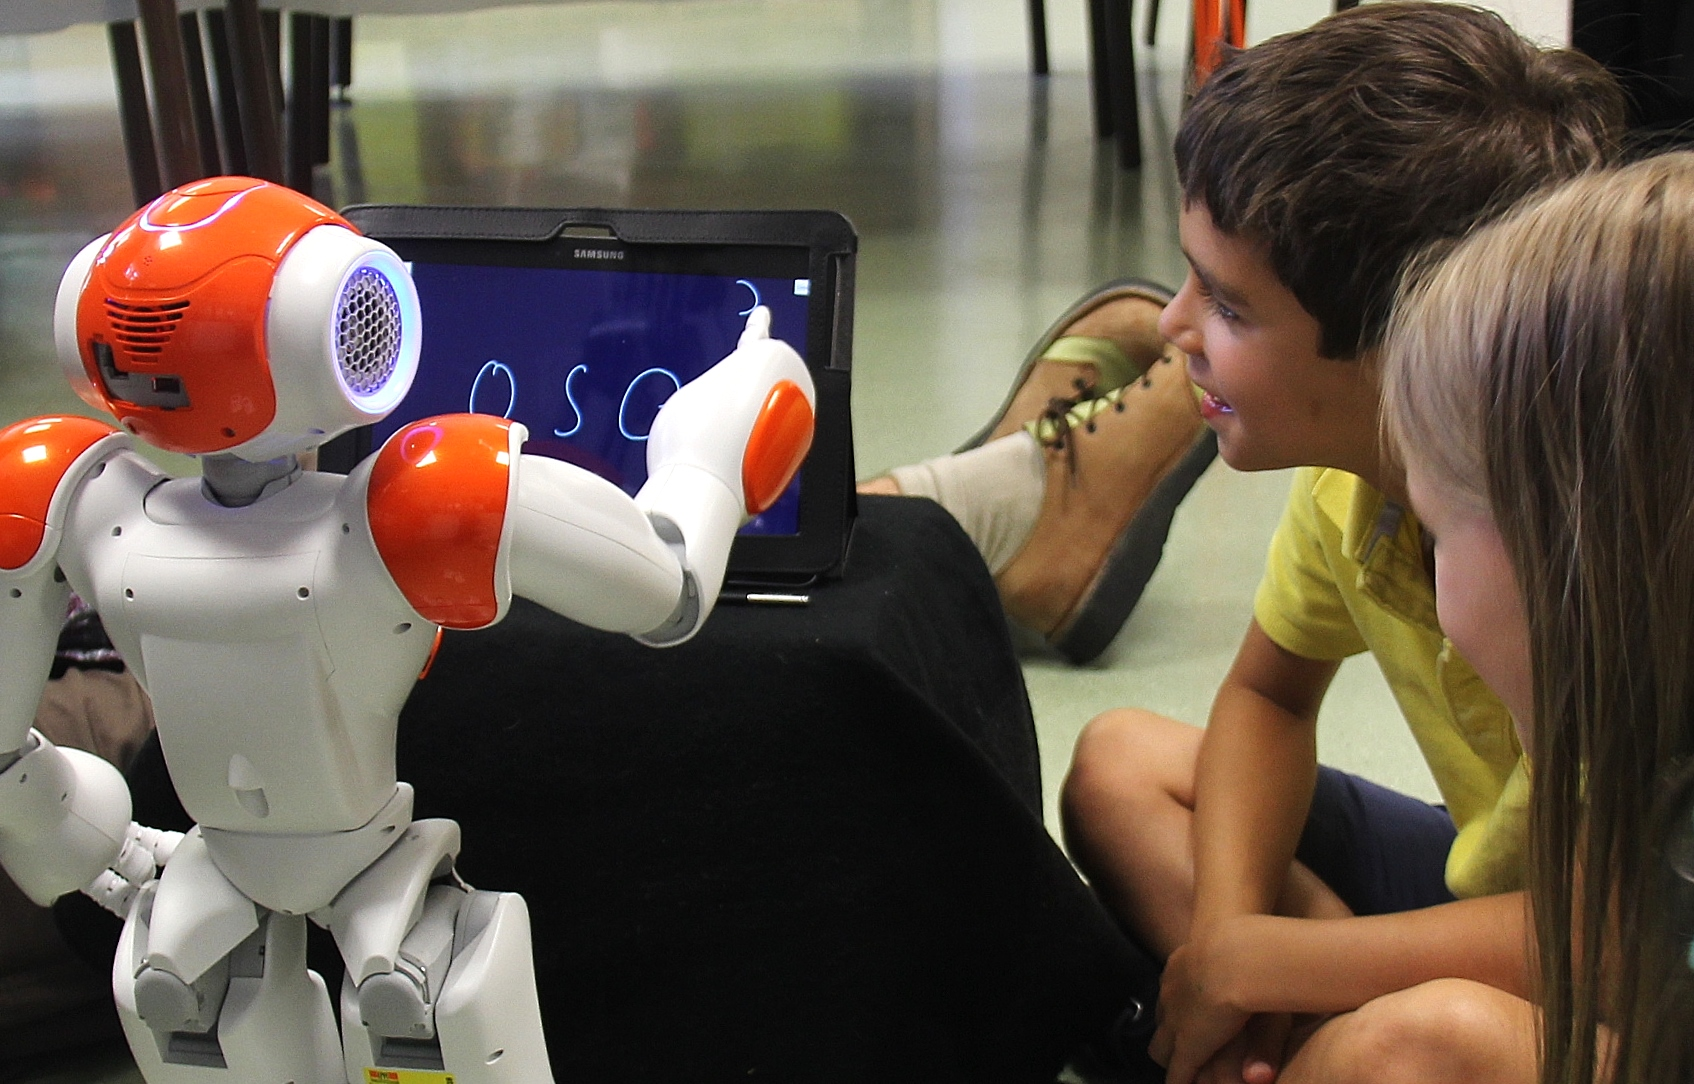
\includegraphics[width=0.9\columnwidth]{cowriter}
        \caption{\textbf{CoWriter}: Children interactively teaching a Nao how to
        write.}
        \label{expe-cowriter}
\end{figure}

\subsubsection{CoWriter} The {\sc CoWriter} project~\cite{hood2015when}
(Figure~\ref{expe-cowriter}) involves a Nao robot and young students
in a \emph{learning by teaching} interaction: the children have to teach the
robot how to write. This experiment involved a dual ROS/NAOqi environment,
bridged within \pyRobots{}. The high-level behaviour was implemented as a finite
state machine ({\sc smach}) whose states corresponded to \pyRobots{} actions.
While the execution controller was subsequently simplified (towards a tighter
interaction scenario), this illustrates how \pyRobots{}, relying on the
ubiquitous Python language, can possibly blend into and interact with existing
tools.

\subsubsection{Stress-test in a kindergarten}
\label{croq}

We organized a pilot study in a kindergarten to stress-test the hardware and
software of the Ranger robot~\cite{mondada2014ranger}. The Ranger robot is an
autonomous robot designed for interaction with children. As it was primarily
designed to support children with tidying up, it is shaped as a wooden ``box on
wheels'' (Figure~\ref{expe-nursery}). It features an RGB-D camera, IR sensors, a
range and bearing sensor, a physical front bumper, a scale, a removable pacifier
(used as a soft on/off switch by the children) and is covered with capacitive
tactile panels. The wooden panels hide 186 RGB LEDs, enabling various light
patterns, the two eyes can be fully controlled (2 DoFs pupils and actuated
eye-lids) and the robot can play sounds. Wheel controllers are designed such
that they switch to freewheel as soon as the robot is pushed by the children.
The robot is powered by a Gumstix Overo board (ARM7l) running a custom Linux
image, assisted by three custom microcontroller boards for low-level hardware
interfacing.

All user-facing behaviours are implemented with \pyRobots{},
and the communication with the hardware is abstracted through a mix of ROS
and Aseba~\cite{magnenat2011aseba} nodes.

\begin{figure}
        \centering
        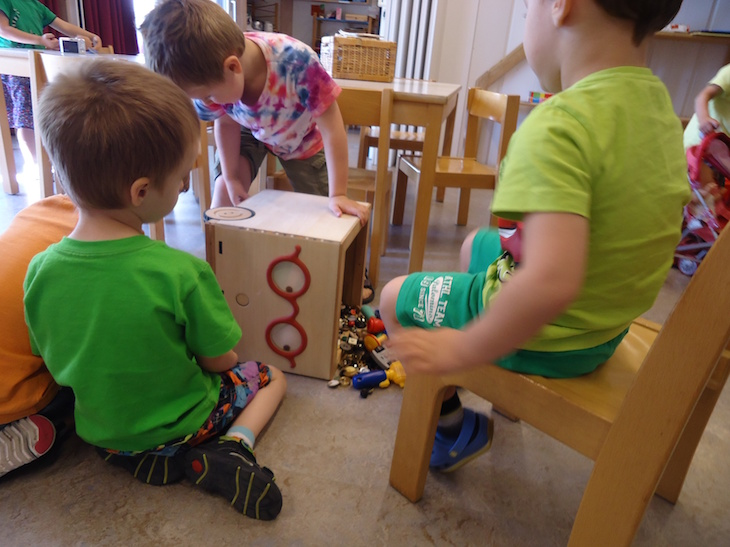
\includegraphics[width=0.9\columnwidth]{ranger-side}
        \caption{\textbf{Stress-test}: Infants playing freely (!) with an EPFL's \emph{Ranger} robot.
        The behaviours of the robot are implemented via \pyRobots{}.}
        \label{expe-nursery}
\end{figure}

We brought two such Ranger robots to a kindergarten (17 children, age: M=3.88,
SD=0.65). After a brief introduction (showing them that removing the pacifier
would ``wake up'' the robot, and putting it back would make it ``fall asleep''),
we invited the children to freely play with the robots and integrate them into
their usual games. The experiment lasted 68 minutes.

We purposefully designed a simple behavioural scheme
(Listing~\ref{croquignole_no_move}): two background actions
(\python|background_blink| and \python|look_at_touches|) run continuously, and 5
events are monitored (pacifier added/removed, toy added/removed and bumper hit).

\begin{listing}[h!]

\begin{pythoncode}
    @action
    def on_pacifier(robot):
        robot.look_at_pacifier()
        robot.blink()
        sleep = robot.fall_asleep()
        robot.lightbar(ramp=colors.RAINBOW).wait()
        sleep.wait()
    
    @action
    def on_pacifier_removed(robot):
        robot.light_bar(colors.from_hls(rand(0,1),0.8,1))
        robot.wakeup().wait()
        robot.move(0.4, v = 0.8).wait()
        robot.idle().wait()
    
    @action
    def on_bumper(robot):
        pulse = robot.pulse_row(0, (128, 0, 128))
        while abs(robot.state.v) > 0.01:
            robot.sleep(0.2)
        pulse.cancel()
    
    @action
    def on_toy(robot):
        robot.playsound(SOUNDS["toy_in"])
        robot.lightbar(ramp=colors.RAINBOW).wait()
    
    with Ranger() as robot:
    
        robot.background_blink()
        robot.look_at_touches()
    
        robot.whenever("pacifier", becomes = True)
                                    .do(on_pacifier)
        robot.whenever("pacifier", becomes = False)
                                    .do(on_pacifier_removed)
        robot.whenever("scale", increase = 0.3).do(on_toy)
        robot.whenever("bumper", becomes = True).do(on_bumper)
    
        while True:
            time.sleep(0.1)
\end{pythoncode}
\caption{Simplified source of the high-level behaviours running on the robots during the
kindergarten study (some behaviours such as the battery management have been omitted for
clarity).}
\label{croquignole_no_move}
\end{listing}

Figure~\ref{croq_actions} shows the average number of events fired and actions
(including sub-actions) started per minute for the whole experiment. The
diagram reveals several peaks above 180 actions/minutes with a global average of
70 actions/minutes, which was surprisingly high considering the simple
behavioural scheme we proposed and the limited actions' depth
($depth_{max}=depth_{\tt look\_at\_touches}=3$) . As a safety measure, we also
set for this study a hard limit to the maximum amount of actions allowed to run
in parallel (20 actions): again, to our surprise, this limit was hit 31 times
during the experiment.

\begin{figure}
    \centering
    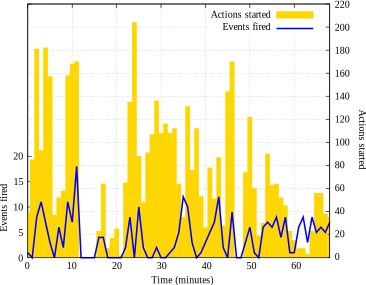
\includegraphics[width=0.9\columnwidth]{croquignole-expe}
    \caption{Events fired and actions started per minute, over the 68min long
    experiment. The robot sustains an average of 70 actions triggered by minute over
    more than an hour, with peaks at 200 actions/minute.}
    \label{croq_actions}
\end{figure}

The results of this stress-test provide a reasonable baseline for the
performance in terms of parallelism and debug/introspection capabilities that
can be expected from an executive controller in a human-robot ``open''
interaction context.

\section{Conclusion and Future Work}


We have presented \pyRobots{}, a novel Python library supporting
development of high-level executive controllers for robotics.

Its main features include a lightweight, unobtrusive design based on code
annotations; a pre-emptive concurrency model allowing for proper, explicit
handling of task cancellation; support for event-based programming; a flexible
robot resource locking mechanism and built-in support for 6D pose
manipulation and transformation.

\pyRobots{} does not aim to replace large execution control frameworks. Instead,
it provides an accessible set of tools to improve upon the all-too-common
\emph{ad-hoc} scripts, while remaining middleware agnostic.

We also report on several experimental deployments on four different
kind of robots using four different middlewares.

Several possible developments would offer interesting perspectives for this
tool, including (a)~the support to suspend (and then resume) actions which
requires defining a satisfying syntax to declare suspend/resume behaviours
within actions; (b)~mechanisms to define action priorities; (c)~investigate
recent work on Python's {\tt asynchio} mechanisms (that provide reference
implementation of co-routines in Python).

Being available as an open-source platform, documented and easy to install, we
believe that these development objectives may be reached soon, as well-defined
use-cases emerge from the library's users.

%%%%%%%%%%%%%%%%%%%%%%%%%%%%%%%%%%%%%%%%%%%%%%%%%%%%%%%%%%%%%%%%%%%%%%%%%%%%%%%%
\section*{Acknowledgments}

This research was supported by the Swiss National Science Foundation through the
National Centre of Competence in Research Robotics.


\bibliographystyle{IEEEtran}
\bibliography{pyrobots}


\end{document}
